\section{Lecture 5: Sampling of signals having Fourier Transform}


\subsection{Sampling}

Ideal sampling is multiplication of the waveform by a uniform train of impulses located at sampling instants.
If $x(t)$ is being sampled, we are multiplying $x(t)$ with $p(t)$ which has impulses located at every sampling instants.
$p(t)$ is shown below.

$$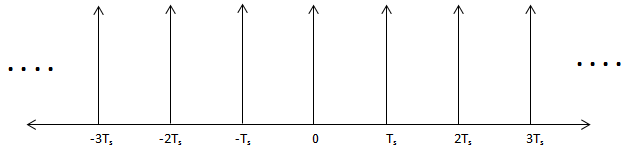
\includegraphics[width=0.5\textwidth]{p_t_.png}$$


Altrnately, we are multiplying original function $x(t)$ by complex fourier expansion of the uniform impulse train.

\subsubsection{Sampling of sinusoid}

Let us focus on one constituent component, or sinusoid in the original waveform $$A_0  \cos ( \frac{2 \pi t}{T_0} + \phi _0 ) $$
Now we are generalizing it to any phase $\phi_0$ unlike we took $\frac{\pi}{4}$ in previous lecture. (Any  $\phi_0 $ will do)

Ideal sampling results in this becoming,
$$ K_0  \left\{ A_0  \cos ( \frac{2 \pi t}{T_0} + \phi _0 )   + \sum_{l=1}^\infty  \left\{  A_0  \cos \left[2\pi(\frac{l}{T_s}-\frac{1}{T_0})t - \phi _0 \right]  +  A_0  \cos \left[2\pi(\frac{l}{T_s}+\frac{1}{T_0})t + \phi _0 \right] \right\} \right\} $$
where $K_0$ is some constant depends on the strength of the impulses.
We have to make sure that all these frequencies are distinct i.e, the imposters do not overlap on original frequencies.As long as $\frac{1}{T_0}$much less than$\frac{1}{T_s}$, all these are distinct frequencies.

Example:  $\frac{1}{T_0} = 1   \mbox{ khz}$, $\frac{1}{T_s} = 20   \mbox{ khz}$
  
  The frequencies are $$\frac{1}{T_0},(\frac{1}{T_s} - \frac{1}{T_0} ),(\frac{1}{T_s} + \frac{1}{T_0}),(\frac{2}{T_s} - \frac{1}{T_0} ),(\frac{2}{T_s} + \frac{1}{T_0})...$$
  
   The frequencies are $ 1,19,21,39,41,...$.Clearly they are distinct!

How small can $\frac{1}{T_s}$ be to keep the frequencies distinct ?
\subsubsection{Keeping imposters distinct}

We are keen on the frequencies being distint because imposters should be distingushable from original waveform.
$$(\frac{1}{T_s} - \frac{1}{T_0} )<(\frac{1}{T_s} + \frac{1}{T_0})$$
We are doubtful if $\frac{1}{T_0}$ and $\frac{1}{T_s} - \frac{1}{T_0}$ are distinct.They are distinct if

 $$(\frac{1}{T_s} -\frac{1}{T_0} )> \frac{1}{T_0}$$
$$\frac{1}{T_s}>\frac{2}{T_0}$$


So,any sampling rate$\frac{1}{T_s}$ greater than(STRICTLY GREATER) twice of original frequency$\frac{1}{T_0}$.That means $\frac{1}{T_s}=3 \mbox{ khz}$ is enough. No need of taking samples at $20 \mbox{ khz}$ frequency.For sampling rate$\frac{1}{T_s}$ the frequencies are $1,2,4,5,7,8,10$.Notice they are still distinct. 

Also note $$\frac{1}{T_s} \neq 2 \mbox{ khz}$$ as $1^{st}$ imposter sits on original waveform.

\subsection{Signals which have and do not have a Fourier transform} 
A waveform or signal is comprised of many sinusoids, the FT of the signal may contain discrete frequencies ( case where $x(t)$ is periodic ), or there can be continuum of frequencies ( when $x(t)$ is aperiodic ).

When we say a waveform is composed of many constituents, we say that waveform has fourier transform.
\subsubsection{Signal having Fourier Transform}

An example of signal that has fourier transform :-

$x(t)=e^{-t}u(t),  
u(t)=$standard unit step



$$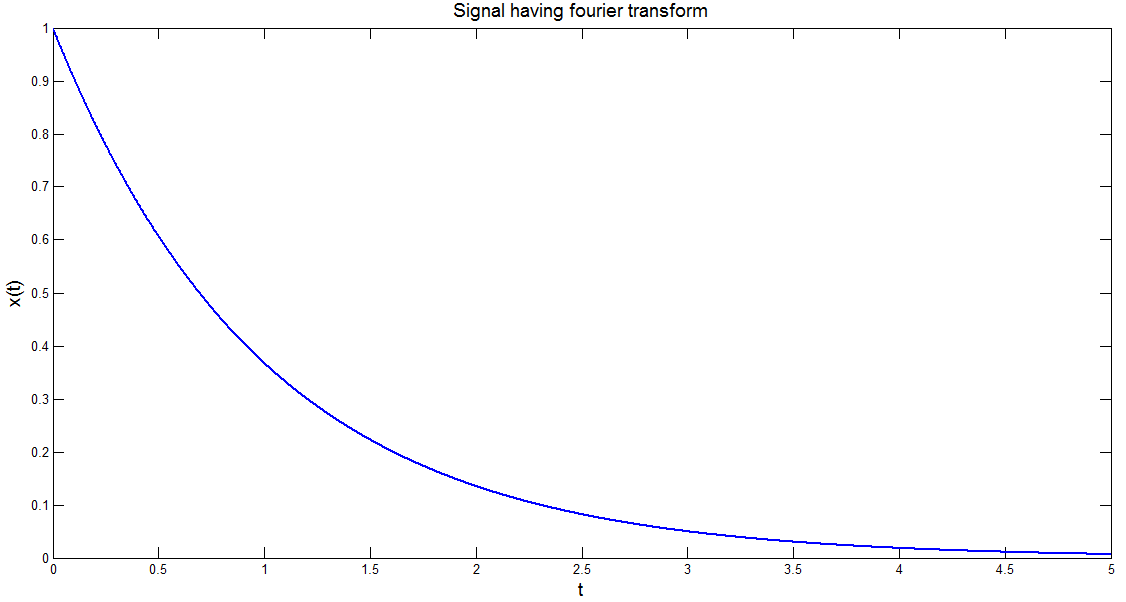
\includegraphics[width=0.6\textwidth]{e_-t.png}$$



$$X(\Omega)= \int_{-\infty}^{+\infty} x(t)e^{-j\Omega t}\mbox{dt}=\int_{-\infty}^{+\infty} e^{-t}e^{-j\Omega t}\mbox{dt}= \int_{-\infty}^{+\infty} e^{-(1+j\Omega t)}\mbox{dt}= \frac{1}{1+j\Omega}$$


$$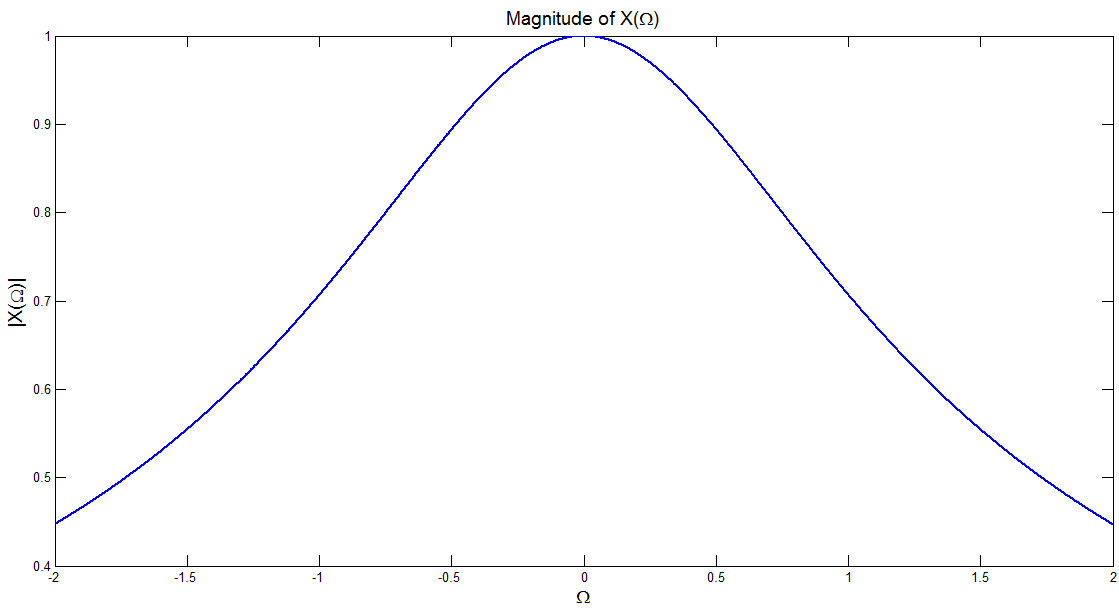
\includegraphics[width=0.6\textwidth]{_X_f__.png}$$

$$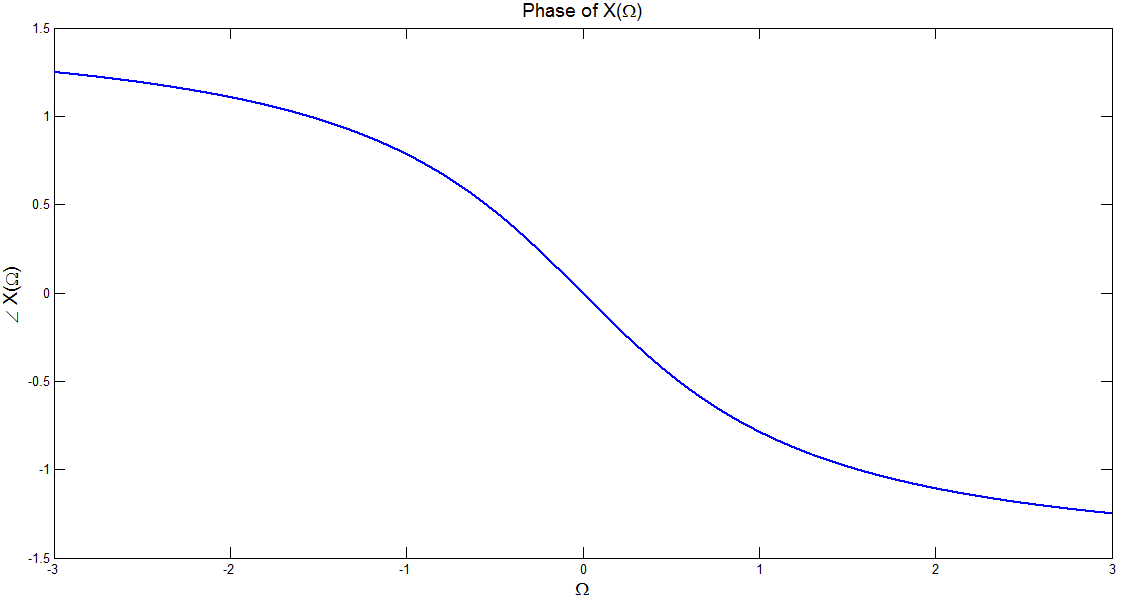
\includegraphics[width=0.6\textwidth]{_lt_X_f_.png}$$


\subsubsection{Signals not having Fourier Transform}

An example for signal which does not have a fourier transform:- 
$y(t)=e^t u(t)$.



$$X(\Omega)= \int_{-\infty}^{+\infty} y(t)e^{-j\Omega t}\mbox{dt}=\int_{-\infty}^{+\infty} e^{t}e^{-j\Omega t}\mbox{dt}$$
$$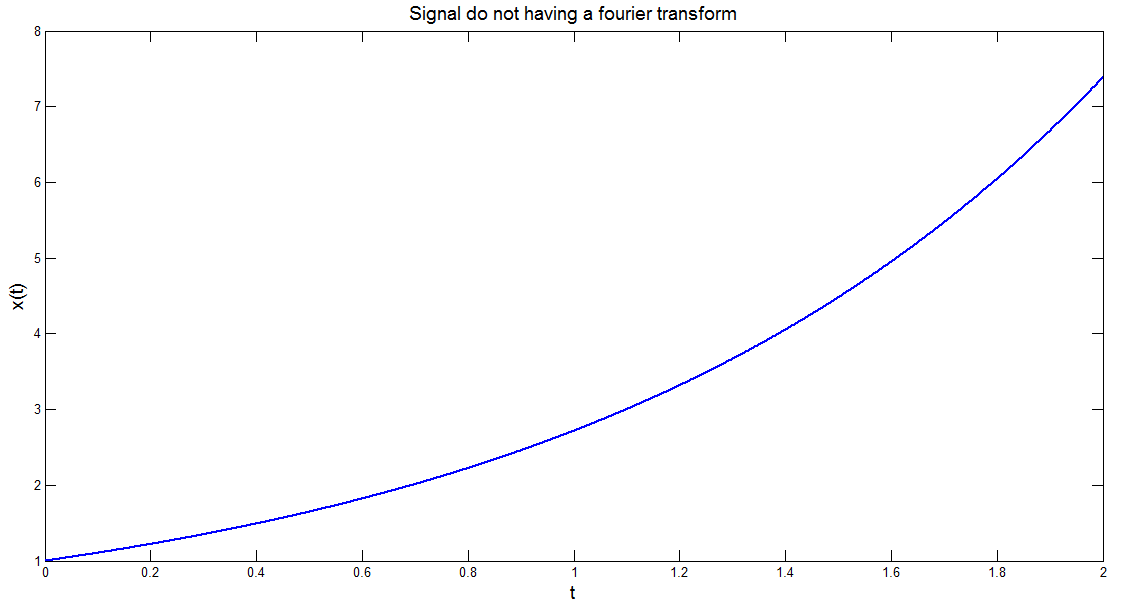
\includegraphics[width=0.6\textwidth]{e_t.png}$$
Clearly the integral doesnot converge.This signal is divergent and so no fourier transform.
Throughout the dicussion on sampling we omit signals which do not have fourier transform from consideration.We only focus on signal having Fourier transform.


$$x(t)=e^{-t}u(t) \iff X(\Omega)=\frac{1}{1+j\Omega}$$

We can reconstruct $x(t)$ from $x(\Omega)$

$$x(t)= \int_{-\infty}^{+\infty} X(\Omega)e^{j\Omega t}\mbox{d}\Omega$$

Recall in the geometric interpretation $X(\Omega)$ is component, $e^{j\Omega t}$ is vector, $\mbox{d}\Omega$ is aggregated over all vector and $\frac{1}{2\pi}$normalizes.

$$X(\Omega)= \overline{X(-\Omega)}$$ $$|X(\Omega)|=|X(-\Omega)|$$
$$ \angle X(\Omega)= - \angle X(-\Omega)$$

Consider  $X(\Omega)e^{j\Omega t} + X(-\Omega)e^{-j\Omega t}$, as one of the constituent.On expansion
$$|X(\Omega)| e ^{j\angle x(\Omega)} e^{j\Omega t} + |X(-\Omega)| e ^{j\angle X(-\Omega)} e^{-j\Omega t}  = 2|x(\Omega)|\{cos(\Omega t + \angle x(\Omega))\mbox{d}\Omega$$ .


We have continuum of such constituents ( $\Omega$ from 0 to $\infty$).



$x(t)$ is combination of $2|X(\Omega)|\{cos(\Omega t + \angle x(\Omega))\}$ for all  $\Omega$.
$$x(t)=\int_0^{\infty}\frac{2}{\sqrt{1+\Omega ^2}}\cos(\Omega t - \tan^{-1}\Omega)$$Note that for every $\Omega \neq 0$, we designed our constituent as combination of $\Omega$ and $-\Omega$ terms. Hence limits vary from $0$ to $\infty$.
Now, when we sample $x(t)$ each and every such constituent is sampled and creates its own imposters.Can we keep all those imposters distinct from original frequencies ? Can we ever sample "adequately" so that we can distinguish imposters from original frequencies?
\subsection{Linearity of sampling}
Recall constituent frequency $\frac{1}{T_0}$, sampling frquency $\frac{1}{T_s}$. Frequencies created in sampling are $$\frac{1}{T_0},\frac{1}{T_s}-\frac{1}{T_0},\frac{1}{T_s}+\frac{1}{T_0} ,\frac{2}{T_s}-\frac{1}{T_0},\frac{2}{T_s}+\frac{1}{T_0} , \cdots$$

The smallest $\frac{1}{T_s}$ we could use is $> \frac{2}{T_0}$ where $\frac{1}{T_0}$ was frequency of one constituent.

When we have combination of sinusoids, can we generalize constituent role ? 
Here a basic question arises: IS SAMPLING LINEAR?

Yes.
Sampling ideally means multiplying the signal by a uniform train of impulse.

sampling of $x(t)$ is $x(t)p(t)$

$$x_1(t) \Rightarrow x_1(t)p(t)$$ sampled at rate $\frac{1}{T_s}$

$$x_2(t) \Rightarrow x_2(t)p(t)$$ sampled at rate $\frac{1}{T_s}$
Now consider a linear combination of $x_1(t)$ and $x_2(t)$

$$\alpha x_1(t) + \beta x_2(t) \Rightarrow \{\alpha x_1(t)+ \beta x_2(t)\}p(t) =\alpha \{x_1(t)p(t)\}+ \beta \{x_2(t)p(t)\} $$

Sampling a linear combination is equivalent to the some linear combination of samples.

Sampling any one of the constituents would create imposters $\frac{1}{T_0},\frac{1}{T_s}-\frac{1}{T_0},\frac{1}{T_s}+\frac{1}{T_0} ,\frac{2}{T_s}-\frac{1}{T_0},\frac{2}{T_s}+\frac{1}{T_0} , \cdots$
For every $T_0$ it will happen.

Effect of sampling a signal with multiple constituents $\cong$ sum of effects of sampling each constituents.

Example : Let us have two constituent frequencies in the original waveform $\frac{1}{T_{0_1}}$ ,$\frac{1}{T_{0_2}}$ $@$ sample rate  $= \frac{1}{T_s}$


The imposters are as follows  $$\frac{1}{T_s}-\frac{1}{T_{0_1}},\frac{1}{T_s}-\frac{1}{T_{0_2}} ,\frac{1}{T_s}+\frac{1}{T_{0_1}},\frac{1}{T_s}+\frac{1}{T_{0_2}} ,\frac{2}{T_s}-\frac{1}{T_{0_1}},\frac{2}{T_s}-\frac{1}{T_{0_2}} ,\frac{2}{T_s}+\frac{1}{T_{0_1}},\frac{2}{T_s}+\frac{1}{T_{0_2}} , \cdots$$

Is it possible to keep imposters distinguished from constituents for all such constituents?
Obviously the answer in this case is NO.

As our sampling rate is finite, every constituent frequency in your signal needs to be finite otherwise we can never distinguish imposters! We need to limit the constituent frquencies!! 
There must be an upper limit on constituent frequency which is nothing but BAND LIMITED SIGNAL. Sampling must be ``adequate'' or take care of imposter.

If our signal is BAND LIMITED what minimum sampling rate do you think would keep those imposters distinct ? Let us answer this in next lecture .
